\section{Strategies and Justification}
A key idea that our group (and all other groups) used is to separate the strategies based on how many people are on the dance floor. However, some ideas like Hexagonal Packing are used regardless of how many dancers are present. We explain each strategy used and under what situations we used them.
\subsection{Small d - Finding all soulmates}
This is a strategy that all groups eventually converged to for small values of d. We believe that the case where d is small is “solved” in that there is no strategy better than this except for small optimizations. The key idea here is to find all dancers' soulmates. The reasoning behind this is that dancing with your soulmate gets you more points and for small values of d it's optimal to find your soulmates in the least amount of time and then dance with them. Our implementation of this is similar to group 6's implementation.\\
We start by placing the dancers in a spiral around the edges of the dance floor and leaving the centre empty. Whenever a dancer finds its soulmate, the pair leaves the dance area and goes to the centre and continues dancing there forever. \\
Note that for this idea to work, every dancer has to dance with every other dancer, otherwise there would be a possibility that some dancer would not find its soulmate and then the minimum score would be affected by this dancer which would hurt the overall score. \\
\begin{figure}[h]
\center
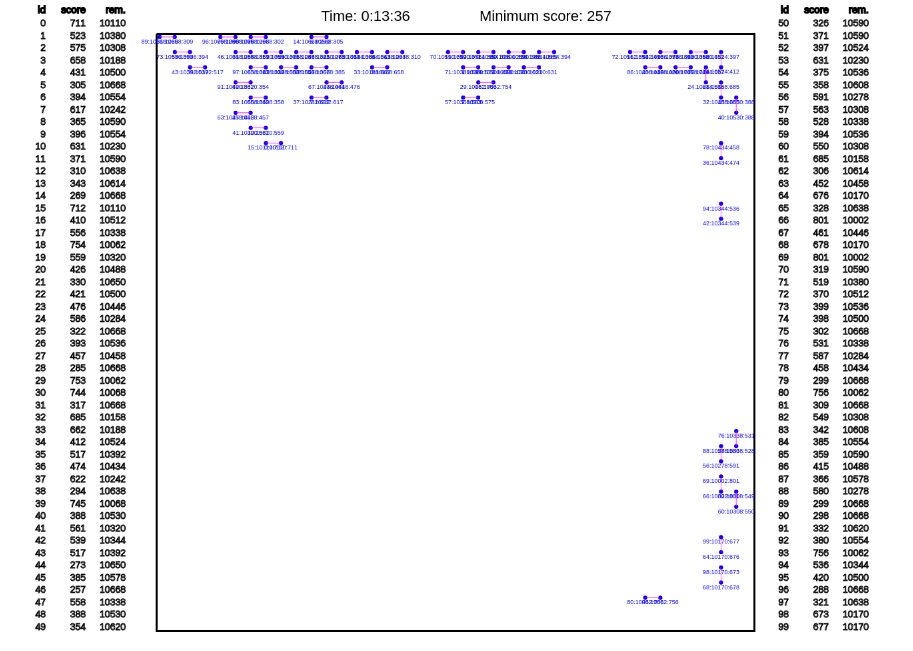
\includegraphics[scale=0.5]{soulmatesfound.png}
\caption{The dance floor after all soulmates have been paired off}
\label{fig:soulmates found}
\end{figure}

\subsubsection{The Basic Implementation}
To do this, we first place the dancers in a pairwise topology, with dancer i paired off with dancer d+1-i. Then we simply move every dancer i to the position of dancer i+1, with dancer d moving to dancer 1's location. It's easy to see that while a lot of pairs do dance together, the only pairs that dance are (i,j) where one of i and j is even and the other is odd. Most groups implemented this for their first deliverable, but our group was one of the two groups (along with group 6) that was able to fix this for our first deliverable with the change shown in the figure.\\
\subsubsection{Making All Pairs Dance}
To make even numbered dancers dance with other evens and odds with odds, we introduce a separate waiting position on the far right. On each step, instead of i going to i+1, only the dancers on the first row move one step to the right. Then we have odds and odds and evens dancing with evens. On the next step, we move the dancer on the waiting position (4 in the figure) and the dancers on the bottom row (except the dancer that is alone) to the location of dancer i+1. The dancer that is alone then moves to the location that was previously the top left corner. This introduces new dancing pairs between every turn of the previous strategy and it is easy to see that a dancer i that danced with a dancer j on one turn will on its next turn dance with dancer j-1. If j = i +1, which means that j-1 = i, on the next turn the dancer will just dance by itself. Since each dancer iterates through all the other dancers, every pair of dancers must eventually dance with each other.\\
Note that this is slightly more efficient if we use a geometry which closes the loop formed by the topology, making 4 and 8 dance with each other. In our current algorithm, on average two dancers do not dance every two turns. This means that the closed loop would only improve the score by a factor of only $\frac{1}{d}$ and we felt that we could improve our strategy in other areas instead.\\
\begin{figure}[h]
\center
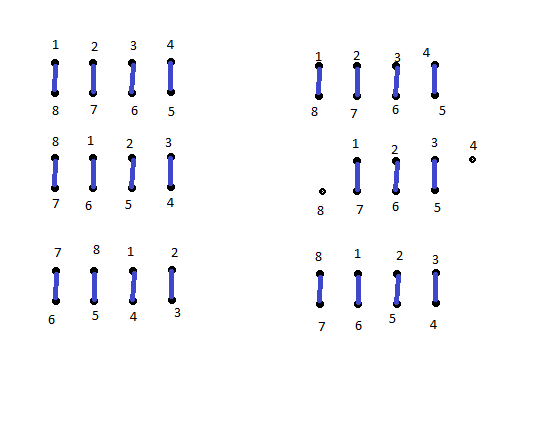
\includegraphics[scale=0.5]{AllDancePairs.png}
\caption{We have three steps. On the left we do not use the fix and only odd-even pairs dance. On the right, we use the fix and even-even pairs and odd-odd pairs also dance}
\label{fig:All pairs dancing}
\end{figure}
\subsubsection{Flattening the Topology}
The difference between our and group 6's deliverable is that they flattened their topology; where two dancers were on opposite sides for our strategy, they were adjacent in group 6's. We later modified our strategy to do the same, because it made modification of the geometry easier to implement.\\
\subsubsection{The Geometry}
Our initial geometry was a circular spiral, because we thought that it would be an efficient way to pack the dancers, but we were wrong and we ended up using a rectangular spiral. The reasoning for a rectangular spiral is that pairs of dancers that have already danced have fewer movements to reach the center where they can dance forever.\\
\subsubsection{Removing Soulmate Pairs}
The final optimization we used was to make dancers who had found their soulmates leave the geometry. Our initial idea was to make all pairs dance and then pair them off. It turned out that removing them as soon as they found their soulmates was faster at pairing them and led to a higher score so we added that in.\\


\begin{figure}[h]
\center
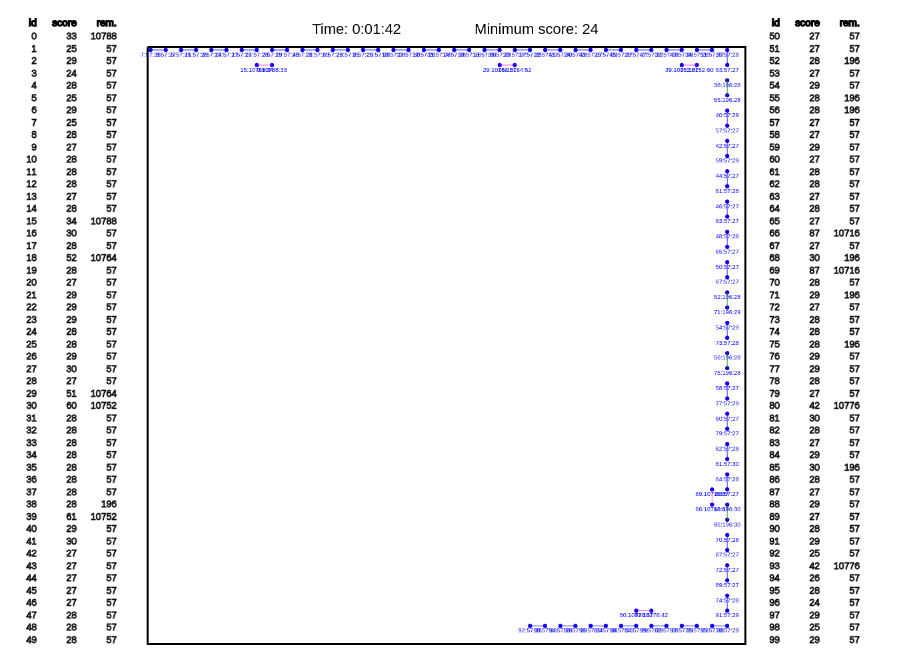
\includegraphics[scale=0.5]{smalld.png}
\caption{}
\label{fig:small d}
\end{figure}

\subsection{Medium d - dance then move}
It is clear that finding all soulmates cannot work for every value of d because there is only limited time and the opportunity cost of searching for soulmates begins to outweigh the potential benefits of finding soulmates. We discuss the exact d that we chose as the upper bound for using the soulmate strategy in the parameter tuning section.\\
\subsubsection{The Main Idea}
The key idea to our strategy is that since it is no longer possible to find everyone's soulmates, it is better to just not try to find soulmates and instead dance as much as possible. The player locations and movement is basically the same as the small d case, except that instead of changing dance partners every turn, we just wait till strangers are tired of dancing and then change dance partners, which basically means we change every 20 turns. An observation here is that since we do not need every pair to dance with each other, we do not have to add the extra waiting position like in small d and just dance only even numbered dancers with odd. Since they change dancers every 20 turns, they dance with a total of 90 different dancers. Since we use our small d strategy well above twice of 90, i.e. 180, we can safely assume that only making evens with odds dance is enough pairs that everyone will have someone to dance with.\\
An interesting feature of this strategy is that the score we get is independent of the value of d. The strategy just involves everyone dancing with a stranger for the entire duration so the score is going to be close to $1800*(3+f)*\frac{20}{21}$ where f is the fraction of friends, which makes (3+f) the expected score per turn and the fraction is because we move every twenty turns. For f = 0, this value is 5142, which would be an upper bound on the score that we could achieve. In fact, we do get a score close to 5000, as we show in the tournament analysis section.\\ 
\subsubsection{Hexagonal Packing}
The upper bound of d for this strategy is simply the number of dancers that can fit on the dance floor in such a way that everyone can dance.\\
Naturally, we can increase this value by using a more efficient packing. We can think of dancers as circles of radius 0.25 because our goal is that no two dancers are at a distance less than 0.5 from each other.\\
The most efficient way to pack circles is with hexagonal packing. As shown in the figure, this takes up less room per row of dancers. For ordinary square packing, we can fit 40 dancers per row and 40 columns for a maximum of 1600 dancers. With hexagonal packing, the space we save allows us to fit 6 more rows of 40 dancers, leading to an upper bound of 1840. This is the largest number of dancers that can dance on the dance floor at one time. We ended up using square packing upto 1600 and then hexagonal packing upto 1840, because our implementation of hexagonal packing had dancers at each end not dancing, which made square packing better if both would fit.\\
\begin{figure}[h]
\center
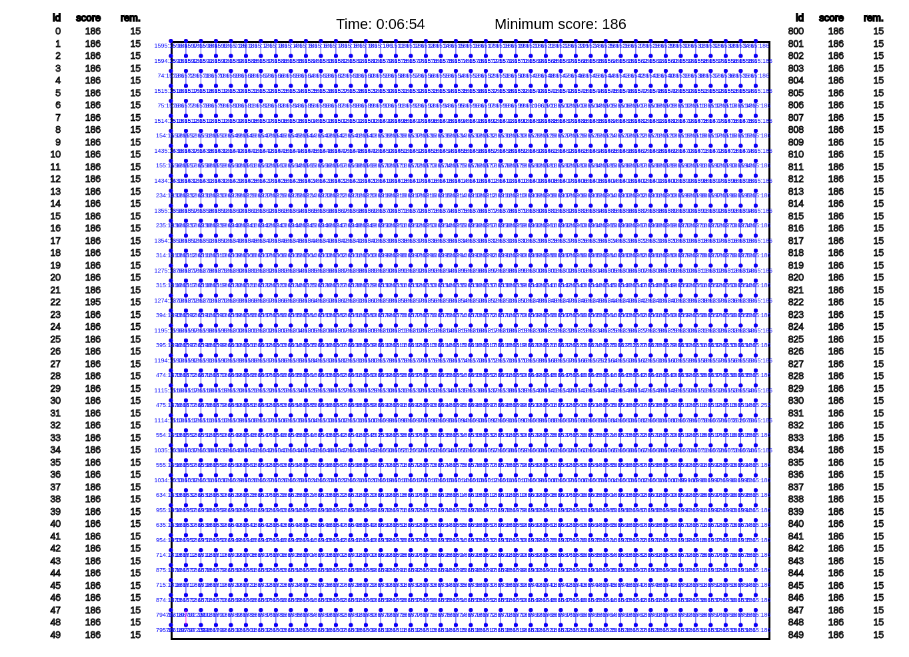
\includegraphics[scale=0.5]{squarepack.png}
\caption{Square packing with 1600 dancers}
\label{fig:Square Packing}
\end{figure}
\\
\begin{figure}[h]
\center
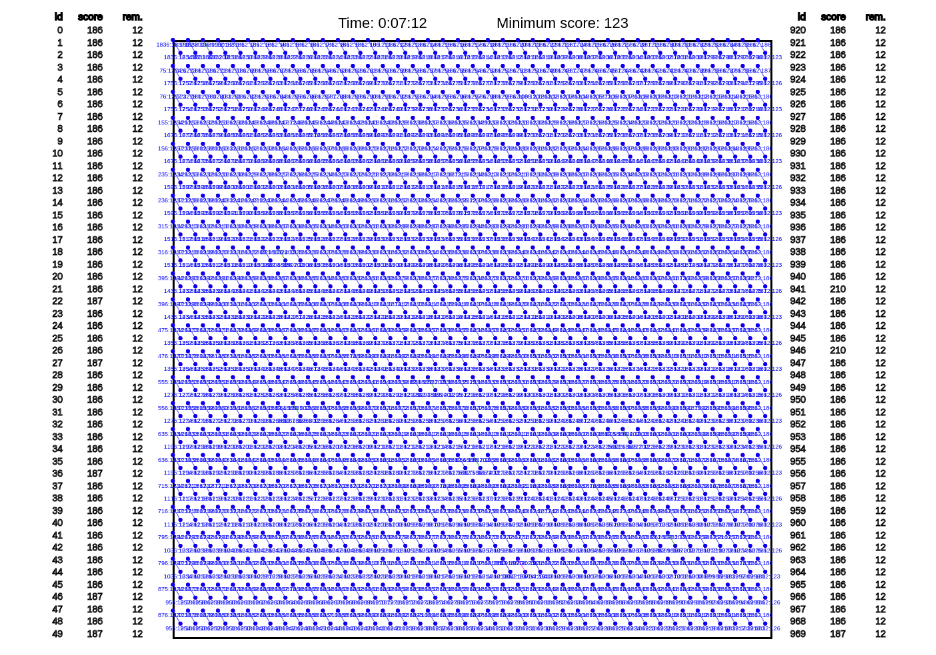
\includegraphics[scale=0.5]{hex.png}
\caption{Hexagonal packing with 1840 dancers}
\label{fig:Hexagonal Packing}
\end{figure}
\subsubsection{Friend Estimation}
On any given turn, we can look at the number of pairs of friends dancing to estimate the true value of f. The probability of a certain dancer dancing with a friend is $\frac{f}{d-1}$, since of the d-1 other dancers, there are f friends. We treat this as a binomial distribution and an estimate for the probability is thus $\hat{f} = \frac{dancers\ dancing\ with\ a\ friend}{d}$. The only problem is that we were unable to find a good way to use it for medium d values.\\